\documentclass[12pt,titlepage]{article}
\usepackage[margin=1.25in]{geometry}
\usepackage{graphicx,amsmath,blindtext,minted}

%% Variables definition
\newcommand{\vSubject}{Data Structure and Algorithm Practicum}
\newcommand{\vSubtitle}{Stack}
\newcommand{\vName}{Muhammad Baihaqi Aulia Asy'ari}
\newcommand{\vNIM}{2241720145}
\newcommand{\vClass}{1I}
\newcommand{\vDepartment}{Information Technology}
\newcommand{\vStudyProgram}{D4 Informatics Engineering}

%% [START] Tikz related stuff
\usepackage{tikz}
\usetikzlibrary{svg.path,calc,shapes.geometric,shapes.misc}
\tikzstyle{terminator} = [rectangle, draw, text centered, rounded corners = 1em, minimum height=2em]
\tikzstyle{preparation} = [chamfered rectangle, chamfered rectangle sep=0.75em, draw, text centered, minimum height = 2em]
\tikzstyle{process} = [rectangle, draw, text centered, minimum height=2em]
\tikzstyle{decision} = [diamond, aspect=2, draw, text centered, minimum height=2em]
\tikzstyle{data}=[trapezium, draw, text centered, trapezium left angle=60, trapezium right angle=120, minimum height=2em]
\tikzstyle{connector} = [line width=0.25mm,->]
%% [END] Tikz related stuff

%% [START] Fancy header related stuff
\usepackage{fancyhdr}
\pagestyle{fancy}
\setlength{\headheight}{15pt} % compensate fancyhdr style
\fancyhead{}
\fancyfoot{}
\fancyfoot[L]{\thepage}
\fancyfoot[R]{\textit{\vSubject - \vSubtitle}}
\renewcommand{\footrulewidth}{0.4pt}% default is 0pt, overline for footer
%% [END] Fancy header related stuff

%% [START] Custom tabular command related stuff
\usepackage{tabularx}
\newcommand{\details}[2]{
    #1 & #2  \\
}
%% [END] Custom tabular command related stuff

%% [START] Figure related stuff
\newcommand{\image}[3][1]{
    \begin{figure}[h]
        \centering
        \includegraphics[#1]{#2}
        \caption{#3}
        \label{#3}
    \end{figure}
}
%% [END] Figure related stuff

%%
\usepackage{pgf-umlcd}

\renewcommand{\umldrawcolor}{black}
\renewcommand{\umlfillcolor}{white}
%%

%% [BEGIN] Custom enumerator
\usepackage{enumitem}
%% [END] Custom enumerator

%% [START] Arab text
\usepackage{arabtex}
\usepackage{utf8}
\usepackage{unicode}
%% [END] Arab Text

%% [BEGIN] Paragraph indent
\usepackage{indentfirst}
%% [END] Paragraph indent

\begin{document}
\begin{titlepage}
    \centering
    \vfill
    {\bfseries\LARGE
        \vSubject\\
        \vskip0.25cm
        \vSubtitle
    }
    \vfill
    
\includegraphics[width=6cm]{images/polinema-logo.png}
    \vfill
    {
        \textbf{Name}\\
        \vName\\
        \vskip0.5cm
        \textbf{NIM}\\
        \vNIM\\
        \vskip0.5cm
        \textbf{Class}\\
        \vClass\\
        \vskip0.5cm
        \textbf{Department}\\
        \vDepartment\\
        \vskip0.5cm
        \textbf{Study Program}\\
        \vStudyProgram
    }
\end{titlepage}

\newpage

\setcounter{section}{1}
\subsection{Learning Objective}
After finishing this practicum session, students will be able to:

\begin{itemize}
    \item Define the Stack Data Structure
    \item Create and implement Stack Data Structure
    \item Implement Stack data Structure with arrays
\end{itemize}

\subsection{Lab Activities}
In this practicum, we will implement \textbf{Stack} class
\subsubsection{Steps}

\begin{enumerate}
    \item Take a look at this following class diagram for \textbf{Stack} class:
    \mbox{}\\
    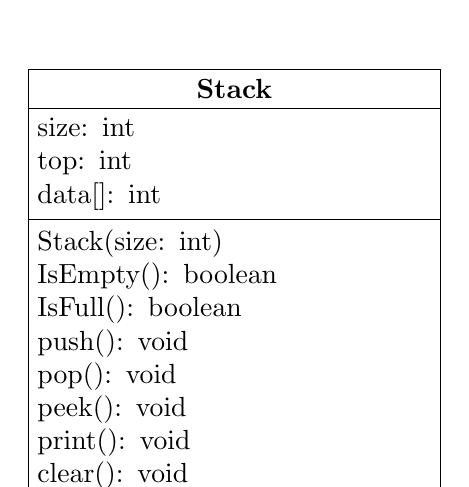
\begin{tikzpicture}
        \begin{class}[text width=5cm]{Stack}{0,0}
            \attribute{size: int}
            \attribute{top: int}
            \attribute{data[]: int}
            \operation{Stack(size: int)}
            \operation{IsEmpty(): boolean}
            \operation{IsFull(): boolean}
            \operation{push(): void}
            \operation{pop(): void}
            \operation{peek(): void}
            \operation{print(): void}
            \operation{clear(): void}
        \end{class}
    \end{tikzpicture}
    \mbox{}\\
    Based on class diagram above, we will create the \textbf{Stack} class in Java program.
    \item Create a new project named \textbf{Jobsheet7}. Create a new package with name \textbf{Practicum1}. Then, create a new class named \textbf{Stack}.
    \item Create new attributes size, top, and data as follows:
    \begin{minted}[autogobble,breaklines]{java}
        int size;
        int top;
        int data[];
    \end{minted}
    \item Add a constructor with parameter as written below:
    \begin{minted}[autogobble,breaklines]{java}
        public Stack(int size) {
            this.size = size;
            data = new int[size];
            top = -1;
        }
    \end{minted}
    \item Create a method \textbf{isEmpty} with Boolean as its return type to check whether the stack is empty or not.
    \begin{minted}[autogobble,breaklines]{java}
        public boolean isEmpty() {
            if (top == 1) {
                return true;
            } else {
                return false;
            }
        }
    \end{minted}
    \item Create a method \textbf{isFull} with Boolean as its return type to check whether the stack is filled completely or not.
    \begin{minted}[autogobble,breaklines]{java}
        public boolean isFull() {
            if (top == size - 1) {
                return true;
            } else {
                return false;
            }
        }
    \end{minted}
    \item Create method \textbf{push} with void as its return type to add new stack element with parameter \textbf{dt}. This dt variable is in form of integer
    \begin{minted}[autogobble,breaklines]{java}
        public void push(int dt) {
            if (!isFull()) {
                top++;
                data[top] = dt;
            } else {
                System.out.println("Stack is full");
            }
        }
    \end{minted}
    \item Create method \textbf{pop} with void as its return type to remove an element from the stack
    \begin{minted}[autogobble,breaklines]{java}
        public void pop() {
            if (!isEmpty()) {
                int x = data[top];
                top--;
                System.out.println("Remove data : " + x);
            } else {
                System.out.println("Stack is empty");
            }
        }
    \end{minted}
    \item Create method \textbf{peek} with void as its return type to check the top element of the stack
    \begin{minted}[autogobble,breaklines]{java}
        public void peek() {
            System.out.println("Top element : " + data[top]);
        }
    \end{minted}
    \item Create method \textbf{print} with void as its return type to display the content of the stack
    \begin{minted}[autogobble,breaklines]{java}
        public void print() {
            System.out.println("Stack content: ");
            for (int i = top; i >= 0; i--) {
                System.out.println(data[i] + " ");
            }
            System.out.println("");
        }
    \end{minted}
    \item Create method \textbf{clear} with void as its data type to remove all elements and make the stack empty
    \begin{minted}[autogobble,breaklines]{java}
        public void clear() {
            if (!isEmpty()) {
                for (int i = top; i >= 0; i--) {
                    top--;
                }
                System.out.println("Stack is now empty");
            } else {
                System.out.println("Failed ! Stack is still empty");
            }
        }
    \end{minted}
    \item Next up, we create a new class named \textbf{StackMain} inside the package \textbf{Practicum1}. Create a main function and make object instantiation with name is \textbf{stk}
    \begin{minted}[autogobble,breaklines]{java}
        public class StackMain {
            public static void main(String[] args) {
                Stack stk = new Stack(5);
            }
        }
    \end{minted}
    \item Fill the stack object by calling method \textbf{push}, the data is being inserted accordingly
    \begin{minted}[autogobble,breaklines]{java}
        stk.push(15);
        stk.push(27);
        stk.push(13);
    \end{minted}
    \item Display the data that we’ve inserted in previous step by calling method \textbf{print}
    \begin{minted}[autogobble,breaklines]{java}
        stk.print();
    \end{minted}
    \item Repeat the insertion process twice, then call pop \textbf{method} to remove an element. We can also check the top data with \textbf{peek} method. Finally, display all the data by calling method \textbf{print}
    \begin{minted}[autogobble,breaklines]{java}
        stk.push(11);
        stk.push(34);
        stk.pop();
        stk.peek();
        stk.print();
    \end{minted}
    \item Compile and run the program, check the result
    \begin{minted}[autogobble,breaklines]{java}
        package Practicum1;

        public class Stack {
            int size;
            int top;
            int data[];

            public Stack(int size) {
                this.size = size;
                data = new int[size];
                top = -1;
            }

            public boolean isEmpty() {
                if (top == 1) {
                    return true;
                } else {
                    return false;
                }
            }

            public boolean isFull() {
                if (top == size - 1) {
                    return true;
                } else {
                    return false;
                }
            }

            public void push(int dt) {
                if (!isFull()) {
                    top++;
                    data[top] = dt;
                } else {
                    System.out.println("Stack is full");
                }
            }

            public void pop() {
                if (!isEmpty()) {
                    int x = data[top];
                    top--;
                    System.out.println("Remove data : " + x);
                } else {
                    System.out.println("Stack is empty");
                }
            }

            public void peek() {
                System.out.println("Top element : " + data[top]);
            }

            public void print() {
                System.out.println("Stack content: ");
                for (int i = top; i >= 0; i--) {
                    System.out.println(data[i] + " ");
                }
                System.out.println("");
            }

            public void clear() {
                if (!isEmpty()) {
                    for (int i = top; i >= 0; i--) {
                        top--;
                    }
                    System.out.println("Stack is now empty");
                } else {
                    System.out.println("Failed ! Stack is still empty");
                }
            }
        }
    \end{minted}
    \begin{minted}[autogobble,breaklines]{java}
        package Practicum1;

        public class StackMain {
            public static void main(String[] args) {
                Stack stk = new Stack(5);

                stk.push(15);
                stk.push(27);
                stk.push(13);

                stk.print();

                stk.push(11);
                stk.push(34);
                stk.pop();
                stk.peek();
                stk.print();
            }
        }
    \end{minted}
\end{enumerate}

\subsubsection{Result}

\begin{minted}[autogobble,breaklines,linenos]{text}
    PS D:\Kuliah>  & 'C:\Program Files\Java\jdk-18.0.2.1\bin\java.exe' '-XX:+ShowCodeDetailsInExceptionMessages' '-cp' 'C:\Users\ASUS\AppData\Roaming\Code\User\workspaceStorage\ ce3fcb236261368a6cbd019dc8ddda8b\redhat.java\ jdt_ws\Kuliah_28156aa7\bin' 'Practicum1.StackMain'
    Stack content: 
    13 
    27
    15

    Remove data : 34
    Top element : 11
    Stack content: 
    11
    13
    27
    15
\end{minted}

\subsubsection{Questions}

\begin{enumerate}
    \item In class \textbf{StackMain}, what is the usage of number 5 in this following code?
    \begin{minted}[autogobble,breaklines]{java}
        Stack stk = new Stack(5);
    \end{minted}
    \item Add 2 more data in the stack with 18 and 40. Display the result!
    \item In previous number, the data inserted in to the stack is only 18 and 40 is not inserted. Why is that?
\end{enumerate}

\subsection{2\textsuperscript{nd} Lab Activities}
In this practicum, we will create a program to illustrate a bunch of books that are stored in Stack. Since the book has some information on it, the stack implementation is done using array of object to represent each element.

\subsubsection{Steps}
\begin{enumerate}
    \item This class diagram is used for creating a program code written in Java programming language
    \mbox{}\\
    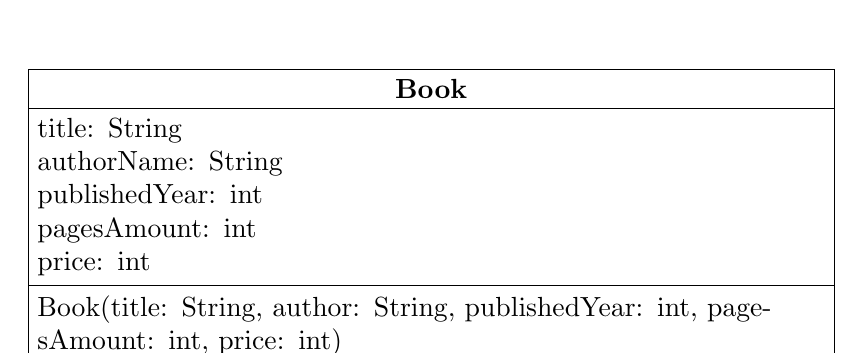
\begin{tikzpicture}
        \begin{class}[text width=10cm]{Book}{0,0}
            \attribute{title: String}
            \attribute{authorName: String}
            \attribute{publishedYear: int}
            \attribute{pagesAmount: int}
            \attribute{price: int}
            \operation{Book(title: String, author: String, publishedYear: int, pagesAmount: int, price: int)}
        \end{class}
    \end{tikzpicture}
    \item Create a new package named \textbf{Practicum2}, then create a new class named \textbf{Book}.
    \item Add attributes in that class, and add the constructor as well.
    \begin{minted}[autogobble,breaklines]{java}
        String title, authorName;
        int publishedYear, pageAmount, price;

        public Book(String tt, String nm, int yr, int pam, int pr) {
            this.title = tt;
            this.authorName = nm;
            this.publishedYear = yr;
            this.pageAmount = pam;
            this.price = pr;
        }
    \end{minted}
    \item Copy the program code for Stack class in \textbf{Practicum1} to be used again in here. Since the data stored in Stack in \textbf{Practicum1} is integer array, and in \textbf{Practicum2} we use objects, we will need to modify some parts in that class.
    \item Modify the Stack class by changing the data type of \textbf{int data[]} to \textbf{Book data[]}. This time we will need to save the data in stack in objects. In addition, we will need to change the \textbf{attributes, constructor, method push}, and \textbf{method pop}
    \begin{minted}[autogobble,breaklines]{java}
        int size, top;
        Book data[];

        public Stack(int size) {
            this.size = size;
            data = new Book[size];
            top = -1;
        }

        public void push(Book dt) {
            if (!isFull()) {
                top++;
                data[top] = dt;
            } else {
                System.out.println("Stack is full");
            }
        }
    \end{minted}
    \item We will need to change the \textbf{print, pop, and peek method} as well since the data that are going to be printed is not only a string, but an object consists of some information (title, authorName, etc.).
    \begin{minted}[autogobble,breaklines]{java}
        public void pop() {
            if (!isEmpty()) {
                Book x = data[top];
                top--;
                System.out.println("Remove data : " + x.title + " " + x.authorName + " " + x.publishedYear + " " + x.publishedYear + " " + x.pageAmount + " " + x.price);
            } else {
                System.out.println("Stack is empty");
            }
        }

        public void peek() {
            System.out.println("Top element : " + data[top]);
        }

        public void print() {
            System.out.println("Stack content: ");
            for (int i = top; i >= 0; i--) {
                System.out.println(data[i].title + " " + data[i].authorName + " " + data[i].publishedYear + " " + data[i].pageAmount + " " + data[i].price);
            }
            System.out.println("");
        }
    \end{minted}
    \item Next, we have to create a new class called \textbf{StackMain} in \textbf{Practicum2}. Create a main function and instantiate an object with named \textbf{st}
    \item Declare the \textbf{Scanner} object with name \textbf{sc}
    \item Insert these lines of codes to receive \textbf{Book} data input, alongside with its information to be stored in stack
    \begin{minted}[autogobble,breaklines]{java}
        Stack st = new Stack(8);
        Scanner sc = new Scanner(System.in);

        char choose;
        do {
            System.out.print("Title : ");
            String title = sc.nextLine();
            
            System.out.print("Author Name : ");
            String name = sc.nextLine();

            System.out.print("Published year : ");
            int year = sc.nextInt();

            System.out.print("Pages Amount : ");
            int pages = sc.nextInt();

            System.out.print("Price : ");
            int price = sc.nextInt();

            Book bk = new Book(title, name, year, pages, price);
            System.out.print("Do you want to add new data to Stack (y/n)? ");
            choose = sc.next().charAt(0);
            sc.nextLine();
            st.push(bk);

        } while (choose == 'y');
    \end{minted}
    \item Call print, pop, and peek method accordingly as follows:
    \begin{minted}[autogobble,breaklines]{java}
        st.print();
        st.pop();
        st.peek();
        st.print();
    \end{minted}
    \item Compile and run \textbf{StackMain}, and observe the result
    \begin{minted}[autogobble,breaklines]{java}
        package Practicum2;

        public class Book {
            String title, authorName;
            int publishedYear, pageAmount, price;

            public Book(String tt, String nm, int yr, int pam, int pr) {
                this.title = tt;
                this.authorName = nm;
                this.publishedYear = yr;
                this.pageAmount = pam;
                this.price = pr;
            }
        }
    \end{minted}
    \begin{minted}[autogobble,breaklines]{java}
        package Practicum2;

        public class Stack {
            int size, top;
            Book data[];

            public Stack(int size) {
                this.size = size;
                data = new Book[size];
                top = -1;
            }

            public boolean isEmpty() {
                if (top == 1) {
                    return true;
                } else {
                    return false;
                }
            }

            public boolean isFull() {
                if (top == size - 1) {
                    return true;
                } else {
                    return false;
                }
            }

            public void push(Book dt) {
                if (!isFull()) {
                    top++;
                    data[top] = dt;
                } else {
                    System.out.println("Stack is full");
                }
            }

            public void pop() {
                if (!isEmpty()) {
                    Book x = data[top];
                    top--;
                    System.out.println("Remove data : " + x.title + " " + x.authorName + " " + x.publishedYear + " " + x.publishedYear + " " + x.pageAmount + " " + x.price);
                } else {
                    System.out.println("Stack is empty");
                }
            }

            public void peek() {
                System.out.println("Top element : " + data[top]);
            }

            public void print() {
                System.out.println("Stack content: ");
                for (int i = top; i >= 0; i--) {
                    System.out.println(data[i].title + " " + data[i].authorName + " " + data[i].publishedYear + " " + data[i].pageAmount + " " + data[i].price);
                }
                System.out.println("");
            }

            public void clear() {
                if (!isEmpty()) {
                    for (int i = top; i >= 0; i--) {
                        top--;
                    }
                    System.out.println("Stack is now empty");
                } else {
                    System.out.println("Failed ! Stack is still empty");
                }
            }
        }
    \end{minted}
    \begin{minted}[autogobble,breaklines]{java}
        package Practicum2;

        import java.util.Scanner;

        public class StackMain {
            public static void main(String[] args) {
                Stack st = new Stack(8);
                Scanner sc = new Scanner(System.in);

                char choose;
                do {
                    System.out.print("Title : ");
                    String title = sc.nextLine();
                    
                    System.out.print("Author Name : ");
                    String name = sc.nextLine();

                    System.out.print("Published year : ");
                    int year = sc.nextInt();

                    System.out.print("Pages Amount : ");
                    int pages = sc.nextInt();

                    System.out.print("Price : ");
                    int price = sc.nextInt();

                    Book bk = new Book(title, name, year, pages, price);
                    System.out.print("Do you want to add new data to Stack (y/n)? ");
                    choose = sc.next().charAt(0);
                    sc.nextLine();
                    st.push(bk);

                } while (choose == 'y');

                st.print();
                st.pop();
                st.peek();
                st.print();
                
                sc.close();
            }
        }
    \end{minted}
\end{enumerate}

\subsubsection{Result}

\end{document}